%!TEX program = xelatex
%%%%%%%%%%%%%%%%%%%%%%%%%%%%%%%%%%%%%%%%%
% Beamer Presentation
% LaTeX Template
% Version 1.0 (10/11/12)
%
% This template has been downloaded from:
% http://www.LaTeXTemplates.com
%
% License:
% CC BY-NC-SA 3.0 (http://creativecommons.org/licenses/by-nc-sa/3.0/)
%
%%%%%%%%%%%%%%%%%%%%%%%%%%%%%%%%%%%%%%%%%

%----------------------------------------------------------------------------------------
%	PACKAGES AND THEMES
%----------------------------------------------------------------------------------------

\documentclass{beamer}

\mode<presentation> {

% The Beamer class comes with a number of default slide themes
% which change the colors and layouts of slides. Below this is a list
% of all the themes, uncomment each in turn to see what they look like.

%\usetheme{default}
%\usetheme{m}
%\usetheme{AnnArbor}
\usetheme{Antibes}
%\usetheme{Bergen}
%\usetheme{Berkeley}
%\usetheme{Berlin}
%\usetheme{Boadilla}
%\usetheme{CambridgeUS}
%\usetheme{Copenhagen}
%\usetheme{Darmstadt}
%\usetheme{Dresden}
%\usetheme{Frankfurt}
%\usetheme{Goettingen}
%\usetheme{Hannover}
%\usetheme{Ilmenau}
%\usetheme{JuanLesPins}
%\usetheme{Luebeck}
%\usetheme{Madrid}
%\usetheme{Malmoe}
%\usetheme{Marburg}
%\usetheme{Montpellier}
%\usetheme{PaloAlto}
%\usetheme{Pittsburgh}
%\usetheme{Rochester}
%\usetheme{Singapore}
%\usetheme{Szeged}
%\usetheme{Warsaw}

% As well as themes, the Beamer class has a number of color themes
% for any slide theme. Uncomment each of these in turn to see how it
% changes the colors of your current slide theme.

%\usecolortheme{albatross}
%\usecolortheme{beaver}
%\usecolortheme{beetle}
%\usecolortheme{crane}
%\usecolortheme{dolphin}
%\usecolortheme{dove}
%\usecolortheme{fly}
%\usecolortheme{lily}
%\usecolortheme{orchid}
%\usecolortheme{rose}
%\usecolortheme{seagull}
%\usecolortheme{seahorse}
%\usecolortheme{whale}
%\usecolortheme{wolverine}

%\setbeamertemplate{footline} % To remove the footer line in all slides uncomment this line
%\setbeamertemplate{footline}[page number] % To replace the footer line in all slides with a simple slide count uncomment this line

%\setbeamertemplate{navigation symbols}{} % To remove the navigation symbols from the bottom of all slides uncomment this line
}

\usepackage{graphicx} % Allows including images
\usepackage{booktabs} % Allows the use of \toprule, \midrule and \bottomrule in tables
\graphicspath{{figures/}}    %设置放置图片的文件夹

\usepackage[boldfont,slantfont]{xeCJK}
\usepackage{fontspec,xunicode,xltxtra}
\setmainfont{Times New Roman}

%for windows fonts
%\setCJKmainfont[BoldFont={SimHei},ItalicFont={KaiTi}]{SimSun}
%\setsansfont{SimHei}
%
%\setCJKfamilyfont{song}{SimSun}
%\setCJKfamilyfont{kai}{KaiTi}
%\setCJKfamilyfont{hei}{SimHei}
%\setCJKfamilyfont{yao}{FZYaoTi}
%
%\newcommand\song{\CJKfamily{song}}
%\newcommand\kai{\CJKfamily{kai}}
%\newcommand\hei{\CJKfamily{hei}}
%\newcommand\yao{\CJKfamily{yao}}

\setCJKmainfont[BoldFont={STXihei},ItalicFont={STKaiti}]{STSong}
\setsansfont{STXihei}
\setsansfont{Monaco}
\setCJKfamilyfont{song}{STSong}
\setCJKfamilyfont{kai}{STKaiti}
\setCJKfamilyfont{hei}{STXihei}
%\setCJKfamilyfont{yao}{FZYaoTi}

\newcommand\song{\CJKfamily{song}}
\newcommand\kai{\CJKfamily{kai}}
\newcommand\hei{\CJKfamily{hei}}
%\newcommand\yao{\CJKfamily{yao}}


\newcommand{\erhao}{\fontsize{22pt}{\baselineskip}\selectfont}
\newcommand{\xiaoerhao}{\fontsize{18pt}{\baselineskip}\selectfont}
\newcommand{\sanhao}{\fontsize{16pt}{\baselineskip}\selectfont}
\newcommand{\xiaosanhao}{\fontsize{15pt}{\baselineskip}\selectfont}
\newcommand{\sihao}{\fontsize{14pt}{\baselineskip}\selectfont}
\newcommand{\xiaosihao}{\fontsize{12pt}{\baselineskip}\selectfont}
\newcommand{\wuhao}{\fontsize{10.5pt}{\baselineskip}\selectfont}
\newcommand{\xiaowuhao}{\fontsize{9pt}{\baselineskip}\selectfont}
\newcommand{\liuhao}{\fontsize{7.5pt}{\baselineskip}\selectfont}

%%%段落首行缩进两个字
% \makeatletter
% \let\@afterindentfalse\@afterindenttrue
% \@afterindenttrue
% \makeatother
% \setlength{\parindent}{2em}%中文缩进两个汉字位

%----------------------------------------------------------------------------------------
%	TITLE PAGE
%----------------------------------------------------------------------------------------

\title{Many-Body Localization in Optical Lattice} % The short title appears at the bottom of every slide, the full title is only on the title page

\author{Bo Xiao} % Your name
\institute[USTC] % Your institution as it will appear on the bottom of every slide, may be shorthand to save space
{
University of Science and Technology of China \\ % Your institution for the title page
\medskip
\textit{xbustc@gmail.com} % Your email address
}
\date{\today} % Date, can be changed to a custom date

\begin{document}
\noindent
\begin{frame}
\titlepage % Print the title page as the first slide
\end{frame}

\begin{frame}
\frametitle{Overview} % Table of contents slide, comment this block out to remove it
\tableofcontents % Throughout your presentation, if you choose to use \section{} and \subsection{} commands, these will automatically be printed on this slide as an overview of your presentation
\end{frame}

%----------------------------------------------------------------------------------------
%	PRESENTATION SLIDES
%----------------------------------------------------------------------------------------

%------------------------------------------------
\section{Quantum Thermalization} % Sections can be created in order to organize your presentation into discrete blocks, all sections and subsections are automatically printed in the table of contents as an overview of the talk
%------------------------------------------------

\subsection{Microcanonical Ensemble} % A subsection can be created just before a set of slides with a common theme to further break down your presentation into chunks

\begin{frame}
\frametitle{Definition}
Isolated System:\\~

\pause No Particle and energy exchange with environment\\~

\pause Conserved energy and particle number

\end{frame}

\begin{frame}
\frametitle{系综理论}
\noindent
系综理论的基本观点:\\~\\
\begin{block}{宏观量的系统时间平均等于系综平均}
$$\overline{u} = <u>_t$$
\end{block}
\end{frame}
% \begin{frame}
% \frametitle{各态遍历假说}
% 系统的运动方程由哈密顿正则方程给出:
% $$\dot{q}_i=\frac{\partial H}{\partial p_i},\dot{p}_i=-\frac{\partial H}{\partial q_i}$$

% 系统状态随时间的变化可以用代表点在相空间中的运动轨道来表示。\\~

% \pause 上述运动方程表明,从不同初态出发系统在相空间内的运动轨道不相交。

% \end{frame}

\begin{frame}
\frametitle{各态遍历假说}
\noindent
玻尔兹曼提出各态遍历假说:\\~

\begin{block}{各态遍历假说}
对于孤立的力学系统,只要时间足够长,系统从任意初态出发,都将经过能量曲面上的一切微观态。
\end{block}
\end{frame}

\begin{frame}{Thermalization}
\noindent

\begin{block}{热力学平衡}
\begin{itemize}
\item 系统的宏观量不再变换,经历所有可能微观状态。
\item 系统的热力学平衡时的统计性质与初态无关。
\end{itemize}
\end{block}
\noindent
\begin{block}{Thermalization}
系统能够进行各态遍历,平衡时宏观量的统计性质与初态无关。
\end{block}
\end{frame}

\begin{frame}{微正则系综宏观量的平衡统计}
\noindent
各态遍历下,对于微正则系综所有可能微观状态出现的概率相同,状态分布在等能面上

$$
{\rho}_n=
\begin{cases}
\frac{1}{\Omega},&E\le E_n \le E+\Delta E\\
0, &\text{other}
\end{cases}
$$
由此可以推导宏观量的热力学平衡期望值
$$\overline{u}=\sum_{n}{\rho_n u_n}$$

\end{frame}
%------------------------------------------------

\subsection{Eigenstate Thermalization Hypothesis(ETH)}
\begin{frame}
\frametitle{为什么要提出ETH?}
量子系统的态在Hamiltonian作用下的含时变化遵循薛定谔方程

$$ i \hbar\frac{\partial \Psi}{\partial t}=H\Psi$$

\pause H是幺正的,量子态的幺正变化无法擦除初态的信息。
\\~

\pause 但是有一类量子系统可以被平衡统计理论表述,平衡态的宏观量大小与初态无关,有着经典统计理论的各态遍历性质,这个被称为Quantum ergodic.
\\~

\pause 为了解释Quantum ergodic,人们提出了Eigenstate Thermalization Hypothesis。

\end{frame}

%------------------------------------------------
\begin{frame}{从宏观量的平衡统计出发}

在能量本征态基矢下,初态$|\Psi>$可以表示为能量本征态的叠加:
$$|\Psi>=\sum_{\alpha}c_{\alpha}|\alpha>$$
\\~

在H作用下随时间变化:
$$|\Psi(t)>=\sum_{\alpha}c_{\alpha}e^{-i E_\alpha t/\hbar}|\alpha>$$
\\~

宏观量在H作用下随时间变化:


$$A(t)=\sum_{\alpha,\beta}c_{\alpha}c_{\beta}^{*}e^{-i(E_\alpha-E_\beta) t/\hbar}A_{\alpha \beta}$$\\

$$=\sum_{\alpha}|c_{\alpha}|^{2}A_{\alpha \alpha}+\sum_{\alpha \ne \beta}c_{\alpha}c_{\beta}^{*}e^{-i(E_\alpha-E_\beta) t/\hbar}A_{\alpha \beta}$$
\end{frame}

\begin{frame}
宏观量的时间平均
$$<A>_t=\frac{1}{\tau}\lim_{\tau \to \infty}\int_{0}^{\tau}A(t)dt $$

$$=\sum_{\alpha}|c_{\alpha}|^{2}A_{\alpha \alpha}+i\hbar\lim_{\tau\to \infty}[\sum_{\alpha\ne\beta}\frac{c_{\alpha}c_{\beta}^{*}A_{\alpha \beta}}{E_\alpha-E_\beta}(\frac{e^{-i(E_\alpha-E_\beta)\tau/\hbar-1}}{\tau})]$$

平衡统计理论下微正则系综的守恒量的时间平均等于系综平均:

$$<A>_{mc}=\sum_{\alpha}{\rho_\alpha A_{\alpha\alpha}}=\frac{1}{N}\sum_{\alpha}{A_{\alpha\alpha}}$$

\pause 如何将上述两个公式等价呢?

\end{frame}

\begin{frame}{ETH的表述}
\noindent
For an arbitrary initial state,  $<\hat{A}>$ will ultimately evolve to its value predicted by a microcanonical ensemble, only small fluctuations around that value, provided that the following two conditions are met:

\begin{itemize}
\item {The diagonal matrix elements $A_{\alpha \alpha }$vary smoothly as a function of energy.}
\item {The off-diagonal matrix elements $A_{\alpha \beta }$, with $ \alpha \neq \beta$ , are much smaller than the diagonal matrix elements.}
\end{itemize}

\end{frame}

\begin{frame}
在两个约束条件下,非对角项非常小,为随时间变化的涨落项。

$$<A>_t=\sum_{\alpha}|c_{\alpha}|^{2}A_{\alpha \alpha} \thickapprox A\sum_{\alpha}|c_{\alpha}|^{2}=A$$
微正则系综的结果:
$$<A>_{mc}\thickapprox \frac{1}{N}*N*A=A$$

So,
$$<A>_t=<A>_{mc}$$

\end{frame}

\begin{frame}
违背ETH的系统:
\begin{itemize}
    \item Intergrate System,有着自己的ETH表述,可以在一定条件下热化。
    \item Localized System,无法热化, non-ergodic, Anderson localization, Many-body localization.
    \item ...
\end{itemize}
\end{frame}
% \begin{frame}{Another saying of Thermalization}
% For full system, density matrix does not thermalize under unitary evolution:
% $$\rho(t)\ne\rho_{eq}(T)=Z^{-1}(T)exp(-H/k_B T)$$
% T is dependent on initial energy.\\~

% But subsystems thermalize:
% $$\lim_{t\to\infty,\overline{S}\to\infty}\rho_{S}(t)=\lim_{\overline{S}\to\infty}\rho^{(eq)}_{S}(T)$$
% Full system acts as a reservior for subsystems, this is another statement of thermalization.


% \end{frame}

\subsection{Anderson localization}
\begin{frame}{Introduction}

Proposed by P.W.Anderson

\begin{itemize}
\item First introduced in 1958(Anderson, P. W. (1958).PhysRev.109.1492)

\item suggest the possibility of eletron localization in semiconductor which contains random impurities or defects.

\item Consider single particle without interaction but can hop from one site to another.

\end{itemize}

\end{frame}

\begin{frame}{Quantum Model}

Tight-binding model hamiltonian

$$H = -\sum_{i,j}J_{ij} \hat{a}^{+}_{i}\hat{a}_{j}+\sum_{i}U_{i}\hat{a}^{+}_{i}\hat{a}_{i}$$

uniform $U_{i}$: extended wavefunction(Bloch wave)\\~


random  $U_{i}$: single particle localized wavefunction

\end{frame}
\begin{frame}{Explanation:matter wave interference}
For single particle in lattice,
\begin{itemize}
\item uniform potential: matter wave freely propagation through lattice
\item random potential: destructive interference between initial wave and wave scattered by impurities
\end{itemize}
\begin{figure}
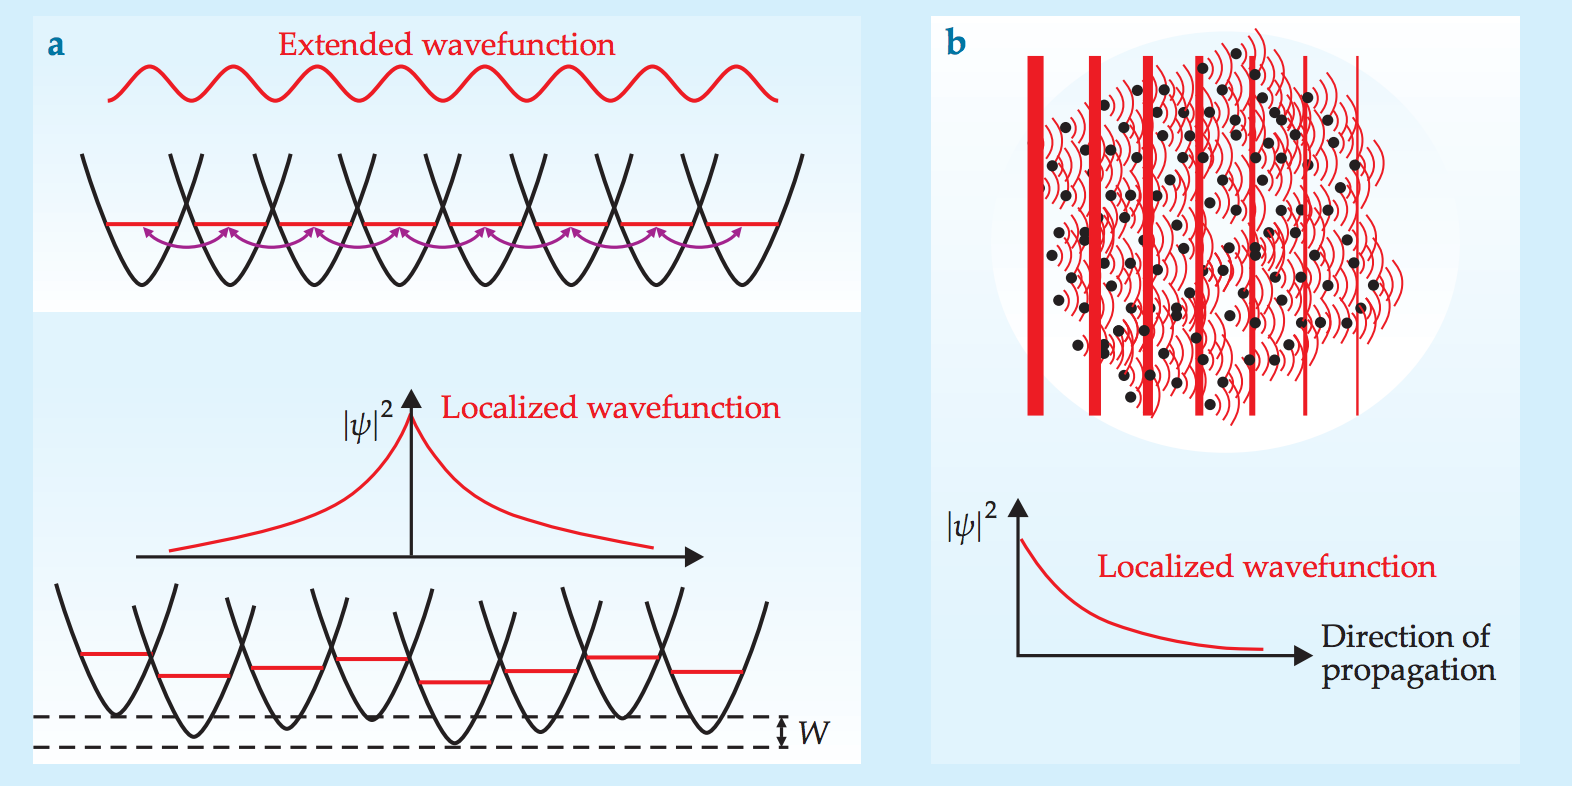
\includegraphics[width=0.6\linewidth]{AndersonLocalization}
\end{figure}
\end{frame}

\begin{frame}{Experiment of Anderson localization in ultracold atoms}
\begin{columns}
\column{0.5\textwidth}
\begin{figure}
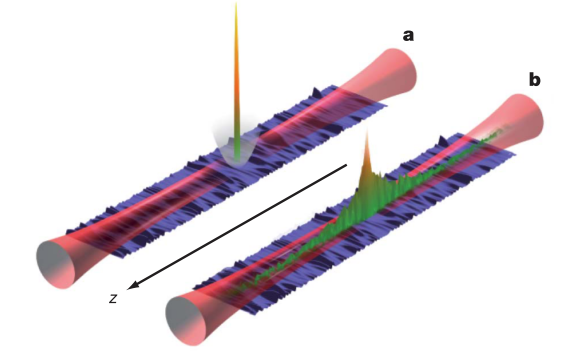
\includegraphics[width=1\linewidth]{adbec}
\end{figure}
\tiny{Anderson localization in non-intereacting 1d BEC\\~

Juliette Billy et.al.Nature 453, 891-894}
\column{0.5\textwidth}
\begin{figure}
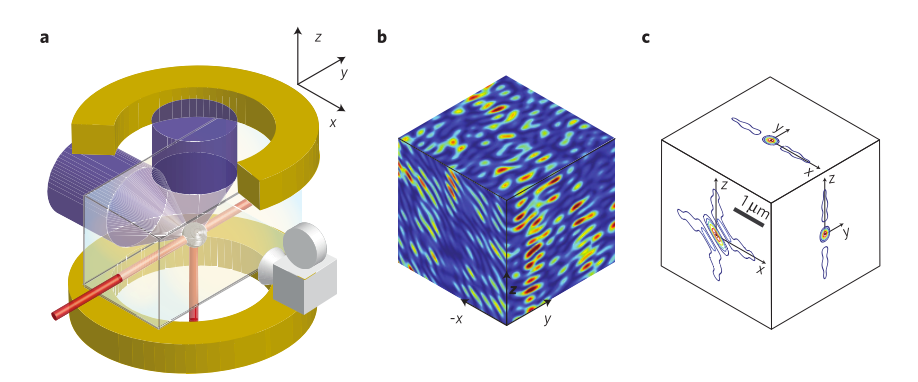
\includegraphics[width=1.1\linewidth]{adlat}
\end{figure}
\tiny{Anderson Localization in 3D ultracold atoms\\~

F. Jendrzejewski et.al.Nature Physics 8, 398–403 (2012)}
\end{columns}

\end{frame}

\begin{frame}{scaling-law theory of anderson localization}

According to scaling-law theory, for models of different dimension system:
\begin{columns}
\column{0.6\textwidth}
\begin{figure}
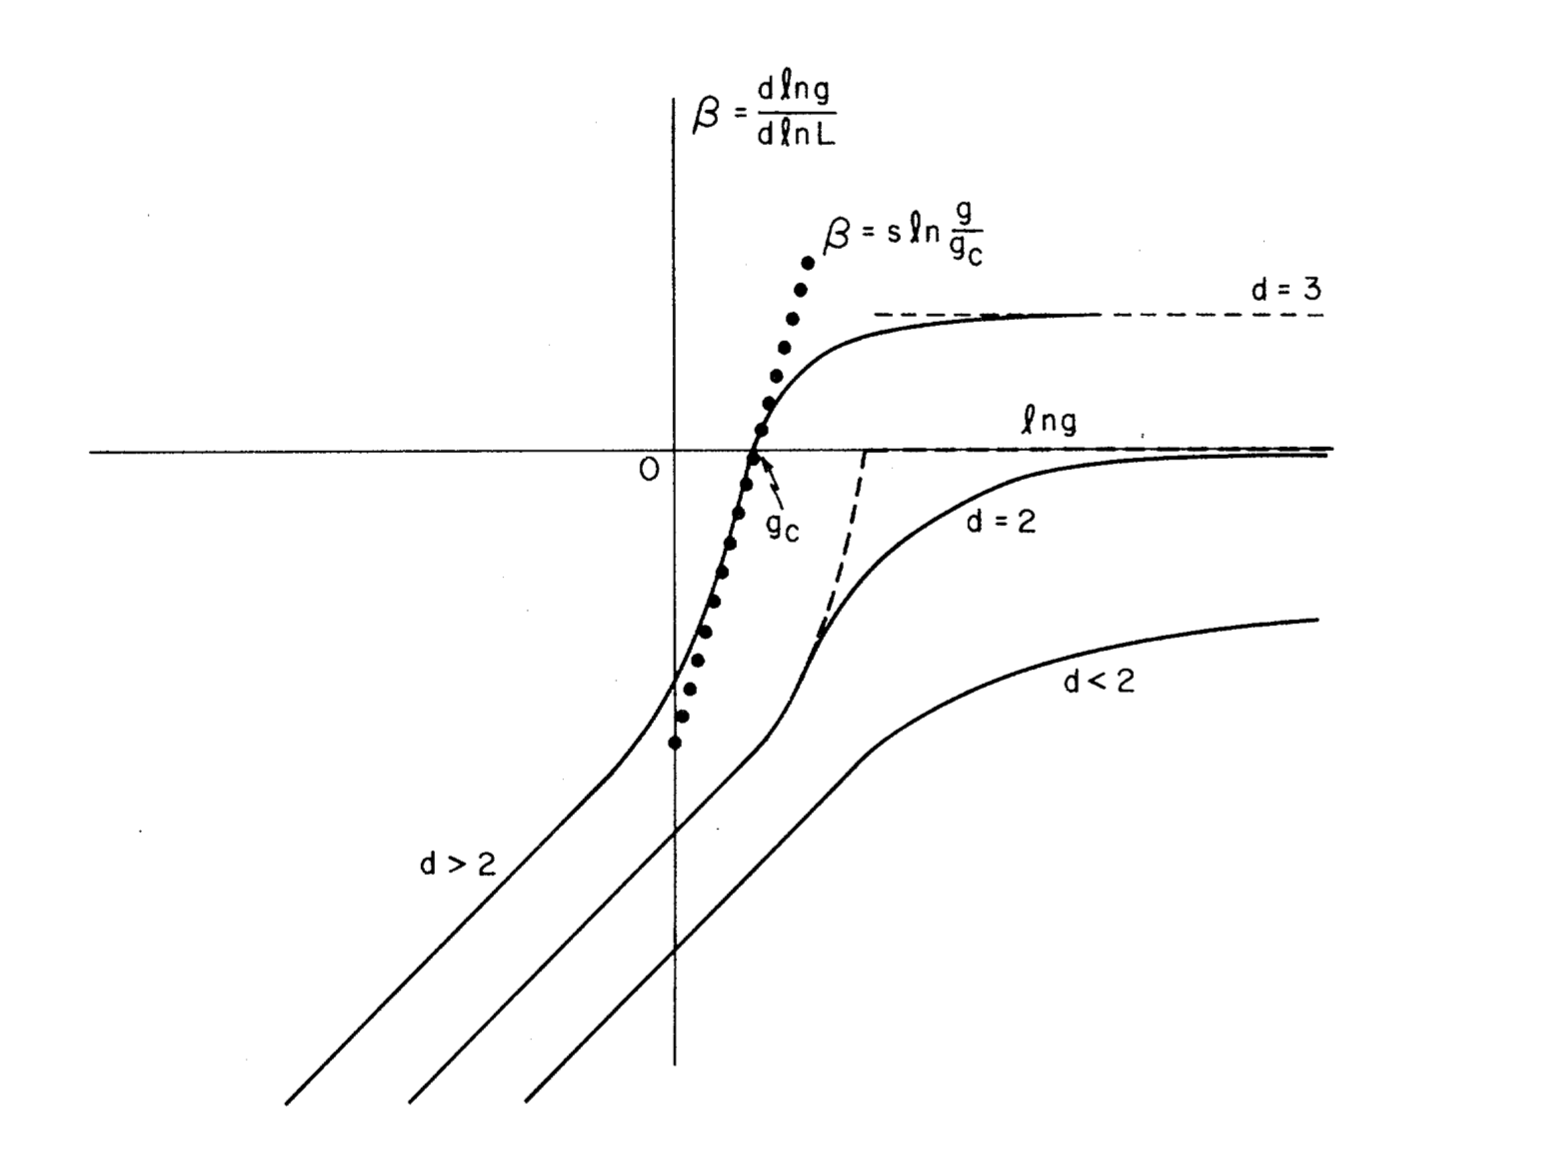
\includegraphics[width=1\linewidth]{scaling}
\end{figure}
\column{0.4\textwidth}
g is conductance,
$$\lim_{g\to\infty}\beta(g)=d-2$$
$$\lim_{g\to0}\beta(g)=log(g)$$

\end{columns}
\end{frame}

\begin{frame}
So, \\~
\begin{itemize}

\item $d\leqslant 2$, system is localized for arbitary weak disorder\\~

\item $d\geqslant 3$, system is localized for some critical disorder strength.
\end{itemize}

\end{frame}


\begin{frame}
Thermalization in anderson localization.

\begin{itemize}

\item Localized states fails to thermalize,violate ETH, so some memory of initial condition is preserved in local observables at long times.

\pause \item Local observables differ from eigenstate to eigenstate in same energy shell.

\end{itemize}

\end{frame}
\subsection{Many-body localization}
\begin{frame}{Many-body localization}

Interaction leads eigenstates to be many-body states due to degree coupling,\\~

Localization with interaction, so called 'Many-body localization'.

\end{frame}
\section{Experiments}
\subsection{one-dimensional quasirandom system}
\begin{frame}
Bloch group:Localization of interacting fermions in a quasirandom optical lattice
\begin{block}{Theoritical Model}
$$\hat{H}=-J\sum_{i,\sigma}(\hat{c}_{i,\sigma}^{\dagger}\hat{c}_{i+1,\sigma}+h.c.)+$$\\~
$$\vartriangle \sum_{i,\sigma}cos(2\pi\beta i+\phi)\hat{c}_{i,\sigma}^{\dagger}\hat{c}_{i,\sigma}+U\sum_{i}\hat{n}_{i,\uparrow}\hat{n}_{i,\downarrow}$$
\end{block}
\end{frame}

\begin{frame}{System Setup and Phase diagram}
$$\beta=\frac{\lambda_s}{\lambda_d}=0.721,\lambda_d= 738nm,Qusirandom!$$
$$Initial\ State:CDW,imbanlance\ I=\frac{N_e-N_o}{N_e+N_o}\thickapprox1 $$
\begin{figure}
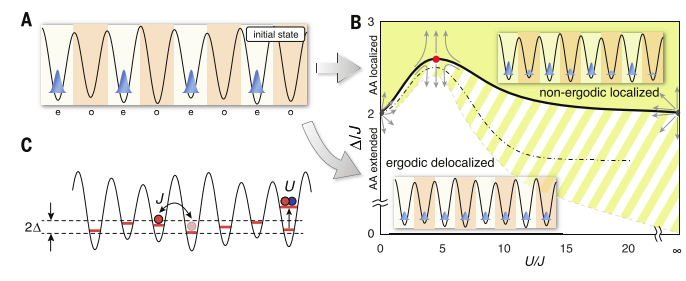
\includegraphics[width=1\linewidth]{Phasediagram}
\end{figure}
\end{frame}

\begin{frame}
\begin{columns}
\column{0.5\textwidth}
\begin{figure}
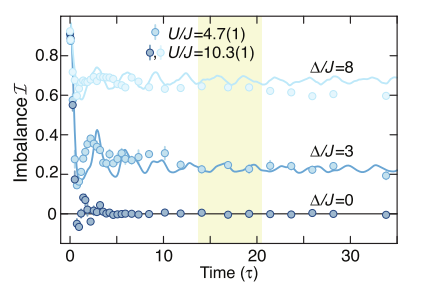
\includegraphics[width=1\linewidth]{lm1.png}
\end{figure}
\column{0.5\textwidth}
\begin{figure}
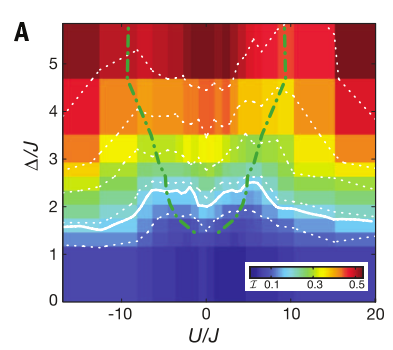
\includegraphics[width=1\linewidth]{lm2.png}
\end{figure}
\end{columns}
~\\
~\\
\rightline{\tiny{Schreiber, M. et.al(2015). Science, 349(6250), 842–845. }}
\end{frame}

\begin{frame}
Coupling identical one-dimensional many-body localized system ,$J_{\perp}:coupling\ between\ tubes$
\begin{block}{Theoritical Model}
$$\hat{H}=-J\sum_{i,j,\sigma}(\hat{c}_{i+1,j,\sigma}^{\dagger}\hat{c}_{i,j,\sigma}+h.c.)-J_{\perp}\sum_{i,j,\sigma}(\hat{c}_{i,j+1,\sigma}^{\dagger}\hat{c}_{i,j,\sigma}+h.c.)+$$\\~
$$\vartriangle \sum_{i,j,\sigma}cos(2\pi\beta i+\phi)\hat{n}_{i,j,\sigma}+U\sum_{i,j}\hat{n}_{i,j,\uparrow}\hat{n}_{i,j,\downarrow}$$
\end{block}
~\\
\rightline{\tiny{Bordia, P. et.al(2016). Physical Review Letters, 116(14), 1–6.}}
\end{frame}

\begin{frame}{System Setup}
\begin{figure}
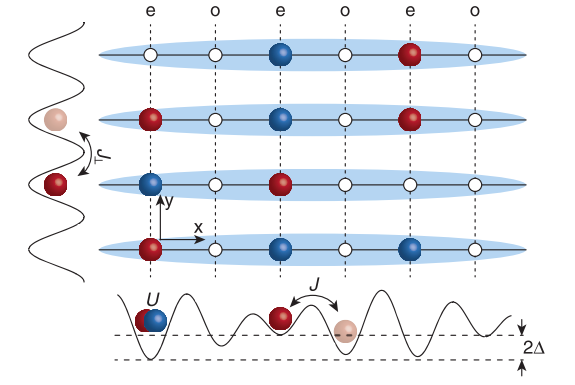
\includegraphics[width=0.8\linewidth]{coupling1}
\end{figure}
\end{frame}

\begin{frame}{Results}
\begin{columns}
\column{0.6\textwidth}
\begin{figure}
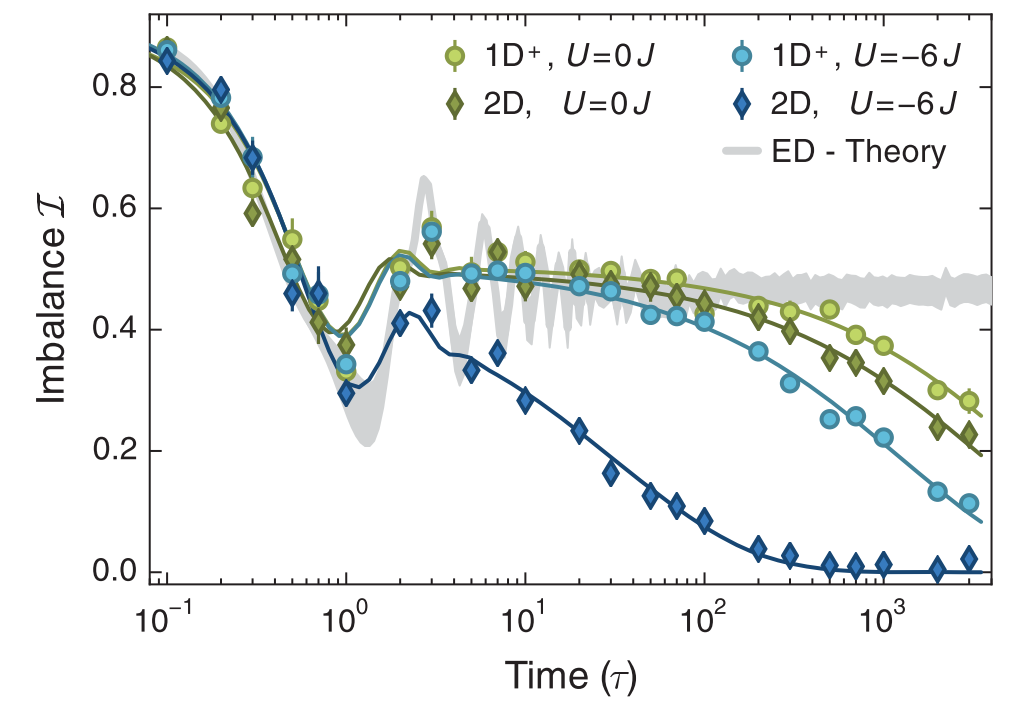
\includegraphics[width=1\linewidth]{coupling2}
\end{figure}
\column{0.4\textwidth}
$$\Delta = 5J$$
$$2D:J_{\perp}=J$$
$$1D^{+}:J_{\perp}\lesssim 10^{-3} J$$
\end{columns}
\begin{center}
\small{non-zero $J_{\perp}$ makes atom can move between tubes free,}\\
\small{with interaction, tubes act as a thermal bath for each other}
\end{center}
\end{frame}

\begin{frame}{Extract Lifetime}
Fitting function:

$$I=(Ae^{-t/t_1}cos(\nu t)+I_{st})e^{-(\Gamma t)^\beta}$$

Imbanlance lifetime:
$$T_{1/e} = 1/\Gamma$$
\begin{figure}
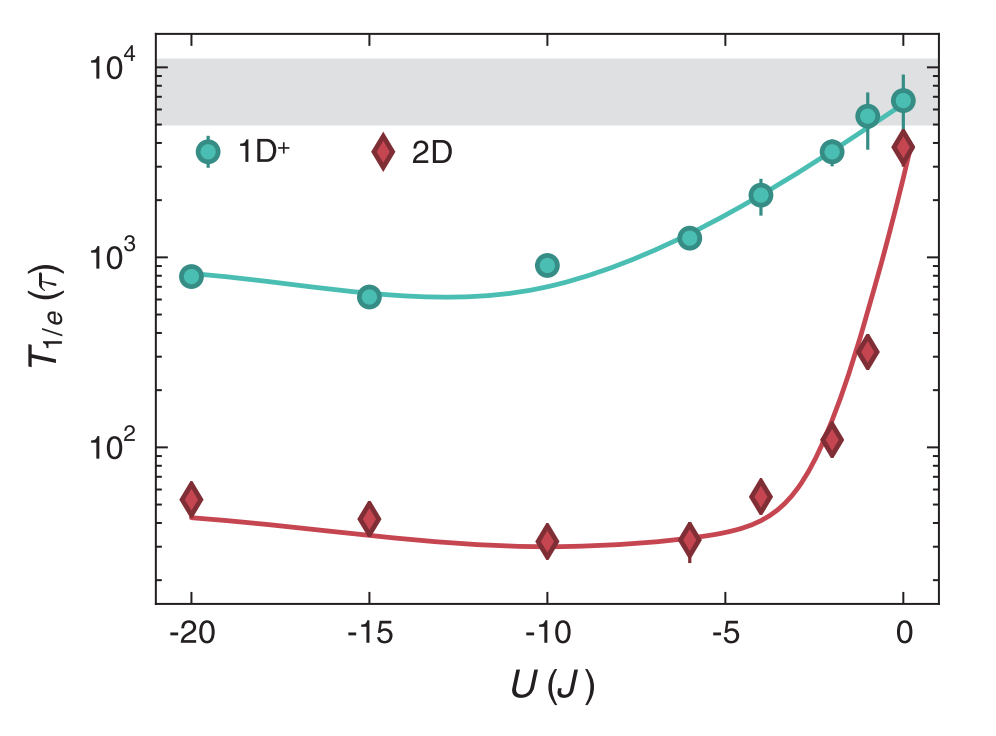
\includegraphics[width=0.5\linewidth]{lifetime}
\end{figure}
\end{frame}

\begin{frame}
Periodically Driving a Many-Body Localized Quantum System,$\nu:modulation\ frequency$
\begin{block}{Theoritical Model}
$$\hat{H}=-J\sum_{i,\sigma}(\hat{c}_{i,\sigma}^{\dagger}\hat{c}_{i+1,\sigma}+h.c.)+$$\\~
$$(\vartriangle+A sin(2\pi\nu t)) \sum_{i,\sigma}cos(2\pi\beta i+\phi)\hat{c}_{i,\sigma}^{\dagger}\hat{c}_{i,\sigma}+U\sum_{i}\hat{n}_{i,\uparrow}\hat{n}_{i,\downarrow}$$
\end{block}
~\\
\rightline{\tiny{Pranjal, B. et.al(2016). arxiv:1607.07868}}
\end{frame}


\begin{frame}{Phase Diagram}
    \begin{figure}
    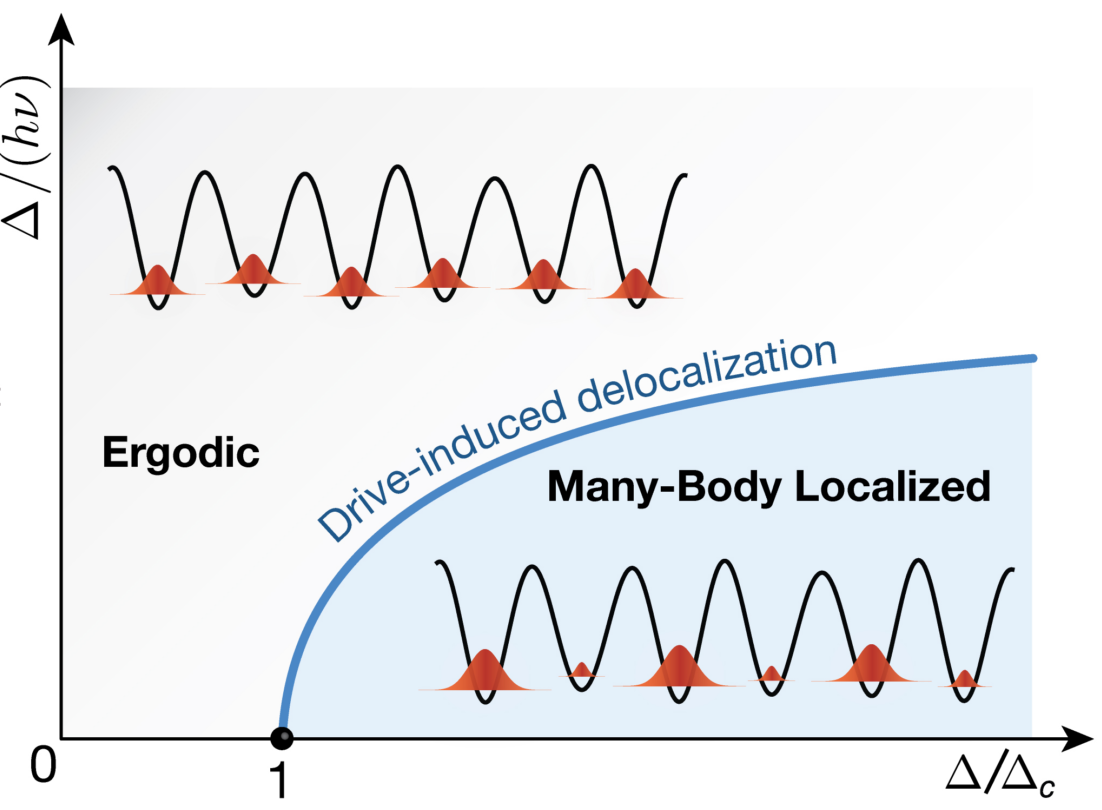
\includegraphics[width=0.8\linewidth]{modulation}
    \end{figure}
\end{frame}

\begin{frame}{Dynamical Response}
  \begin{itemize}
    \item \small{When $\nu$ is small, system can response to the time-dependent Hamilatonian.}
    \item \small{When $\nu$ is large, the dynamics is effectively governed by the time-averaged non-ergodic Hamilatonian.}
  \end{itemize}
    \begin{figure}
    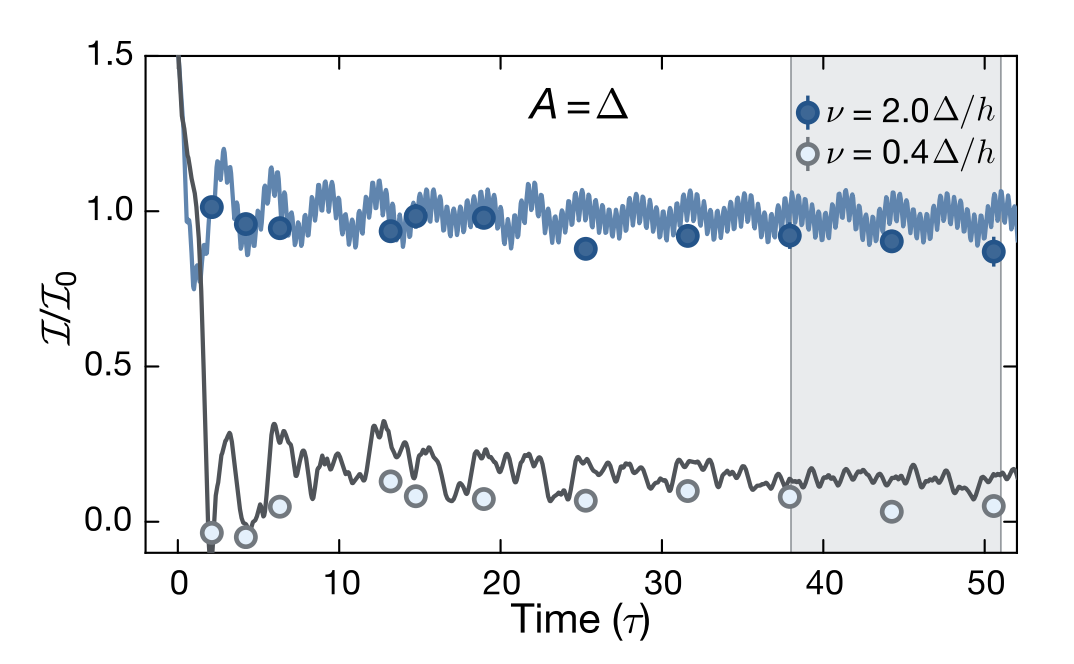
\includegraphics[width=0.8\linewidth]{Moduevolu}
    \end{figure}
\end{frame}

\begin{frame}{Dynamical Phase Diagram}
  \begin{figure}
  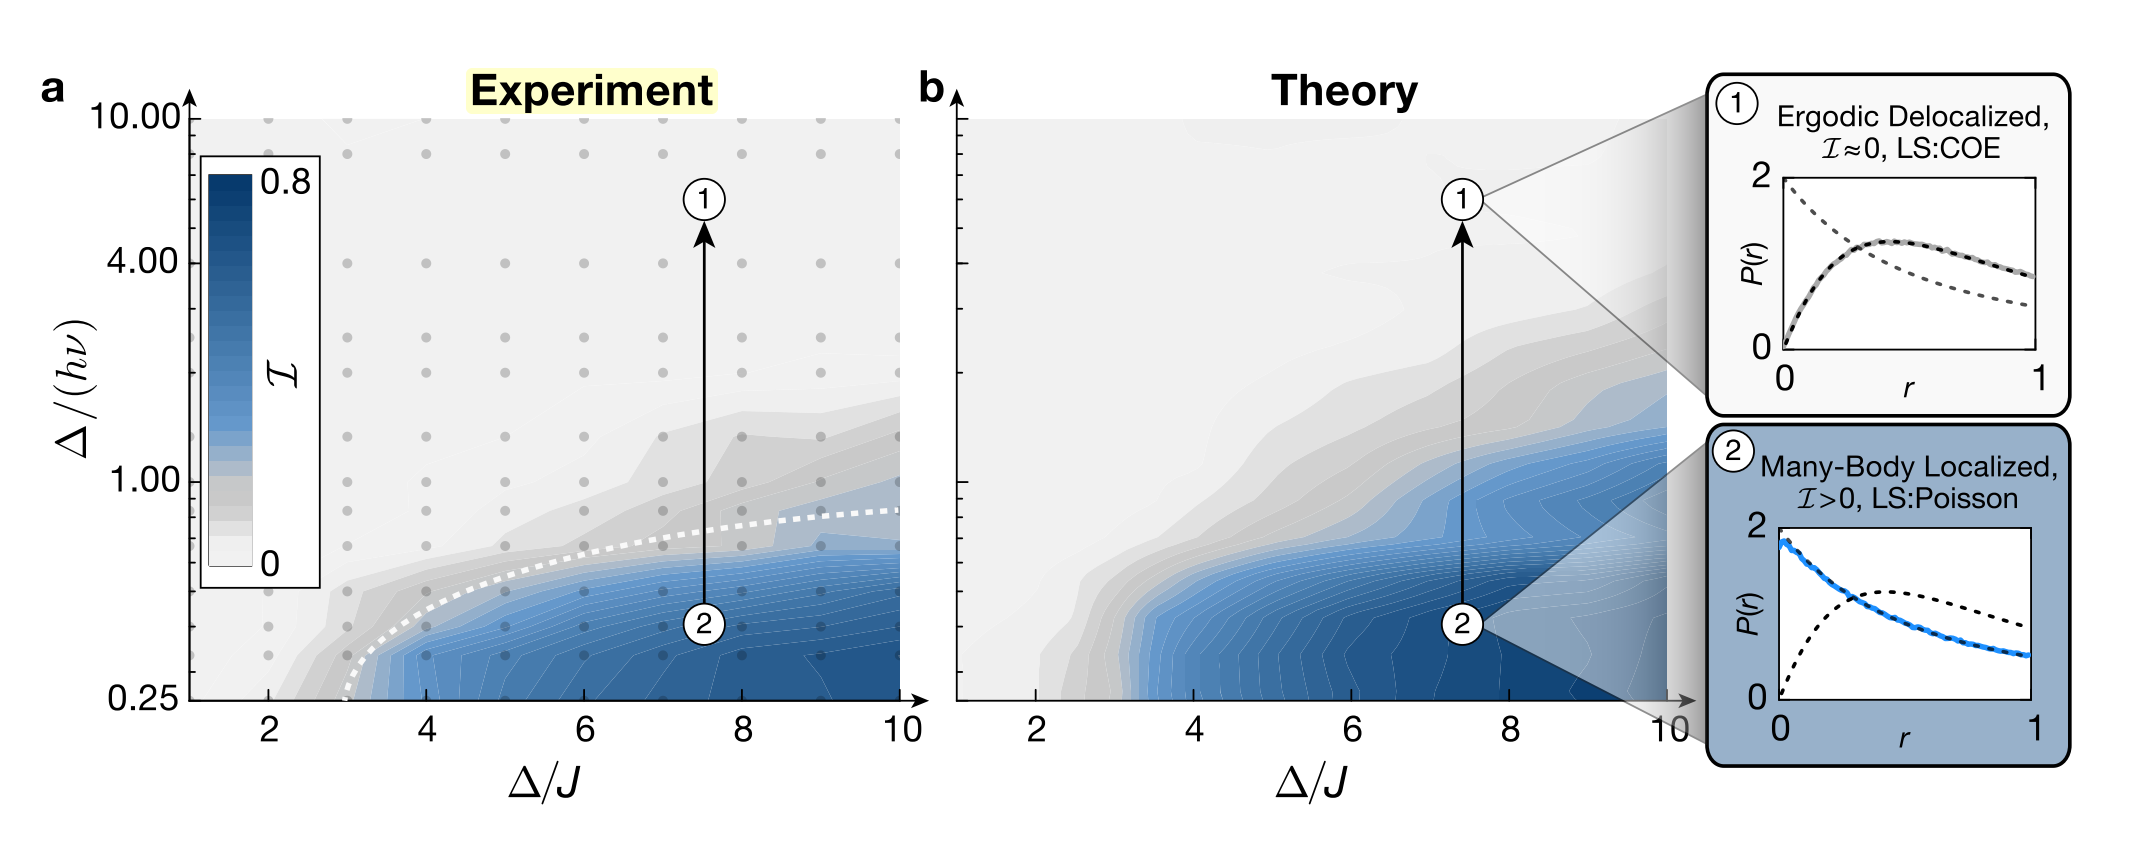
\includegraphics[width=1\linewidth]{Phasegram}
  \end{figure}
\end{frame}

\begin{frame}{Level Statistic}
Define level statistic parameter:
$$r=min[\frac{\epsilon_{\alpha+1}-{\epsilon}_\alpha}{{\epsilon}_\alpha-{\epsilon}_{\alpha-1}},\frac{\epsilon_{\alpha}-{\epsilon}_{\alpha-1}}{{\epsilon}_{\alpha+1}-{\epsilon}_{\alpha}}]$$
Typical distributions of r:
\begin{itemize}
  \item Circular orthogonal ensemble(COE):$$P_{COE}=\frac{2}{3}(\frac{1}{(1+r)^2}+\frac{sin(\frac{2\pi r}{r+1})}{2\pi r^2}$$
  $$+\frac{sin(\frac{2\pi }{r+1})}{2\pi}-\frac{cos(\frac{2\pi }{r+1})}{r+1}-\frac{cos(\frac{2\pi r}{r+1})}{r(r+1)})$$
  \item Possion:$$P_{POI}=\frac{2}{(1+r)^2}$$
\end{itemize}
\end{frame}

\begin{frame}{Level Statistic}
Use the distribution to determine different phases:
\begin{itemize}
\item For MBL phase, there is no level repulsion,eigenstates has large distance and little overlap in Fock space,so Possion Statistic.
\item For ergodic phase, coupling leads to level repulsion,so COE.
\end{itemize}
\end{frame}

\subsection{2-dimension many-body localized system}
\begin{frame}
\begin{center}
  \textbf{Exploring the many-body localization transition in two dimensions}
\end{center}
\end{frame}

\begin{frame}
  \begin{block}{Theoritical Model}
  $$\hat{H}=-J\sum_{<i,j>}(\hat{a}_{i}^{\dagger}\hat{a}_{j})-\frac{U}{2}\sum_{i}(\hat{n}_{i}^{\dagger}(\hat{n}_{i}-1)+\sum_i(\delta_i+V_i)\hat{n}_i^{\dagger}$$
  \end{block}
$\delta:onsite\ random\ potential$
$disorder\ strength\ \Delta:full-width\ half-maximum\ of\ disorder\ distribution$
\end{frame}

\begin{frame}{Experimental Setup}
  \begin{figure}
  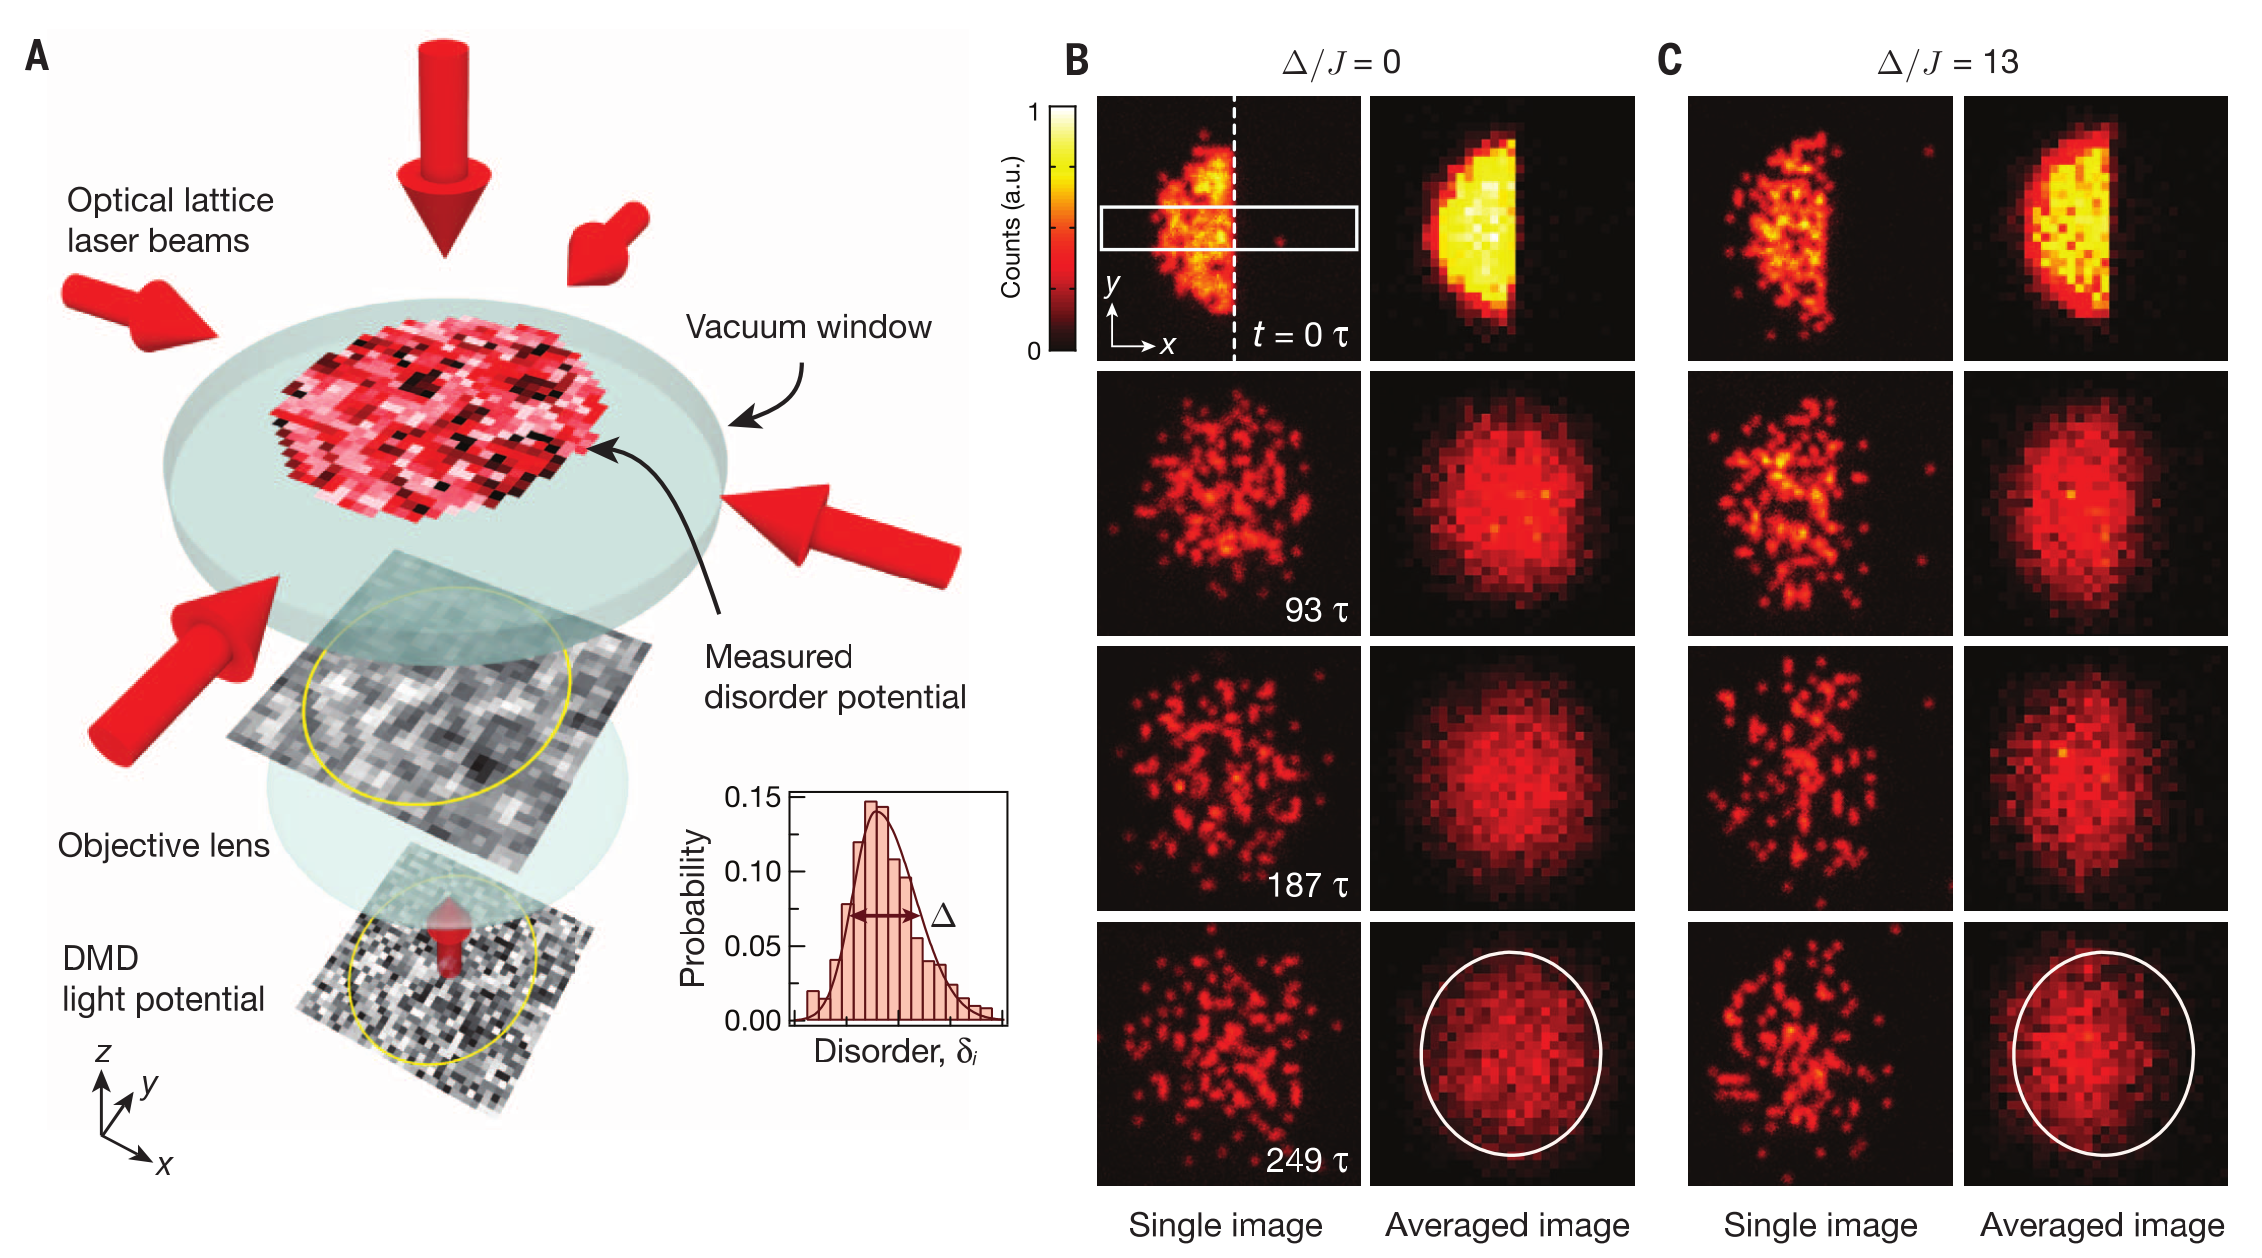
\includegraphics[width=0.8\linewidth]{2dset}
  \end{figure}
  \small{Technique:High resolution Imaging, DMD with 787.5nm laser}\\
  \small{Interaction $U=24.4J, J/h=24.8Hz$}
  \rightline{\tiny{Choi, J. et.al(2016). Science, 352(6293), 1547–1552.}}
\end{frame}

\begin{frame}{Number Imbanlance}
  Use Number Imbalance to identify diffrent phases:
  $$I=\frac{N_L-N_R}{N_L+N_R}$$
  In this experiment, I is meausured in the center region over 5 sites in the y direction.
\end{frame}

\begin{frame}{Dynamics}
  \begin{figure}
  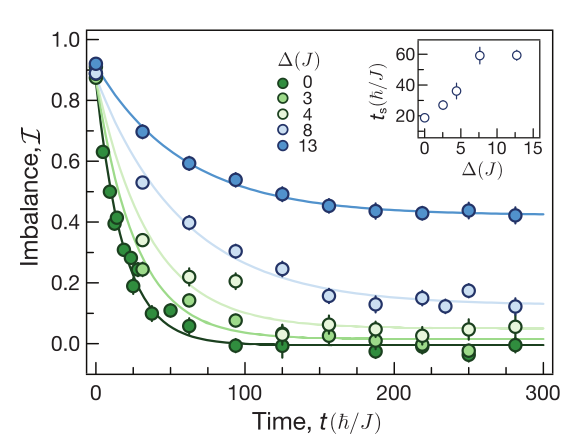
\includegraphics[width=0.8\linewidth]{2ddy}
  \end{figure}
\end{frame}

\begin{frame}{Identify MBL Transition}
\small{$$\delta n =({\sum}_{i}[n_i(0)-n_i(\Delta)]^2)$$}
\small{$$n_i(\Delta)=\frac{1}{5}{\sum}_{j=-2}^{2}n_{i,j}(0)$$}
\begin{figure}
 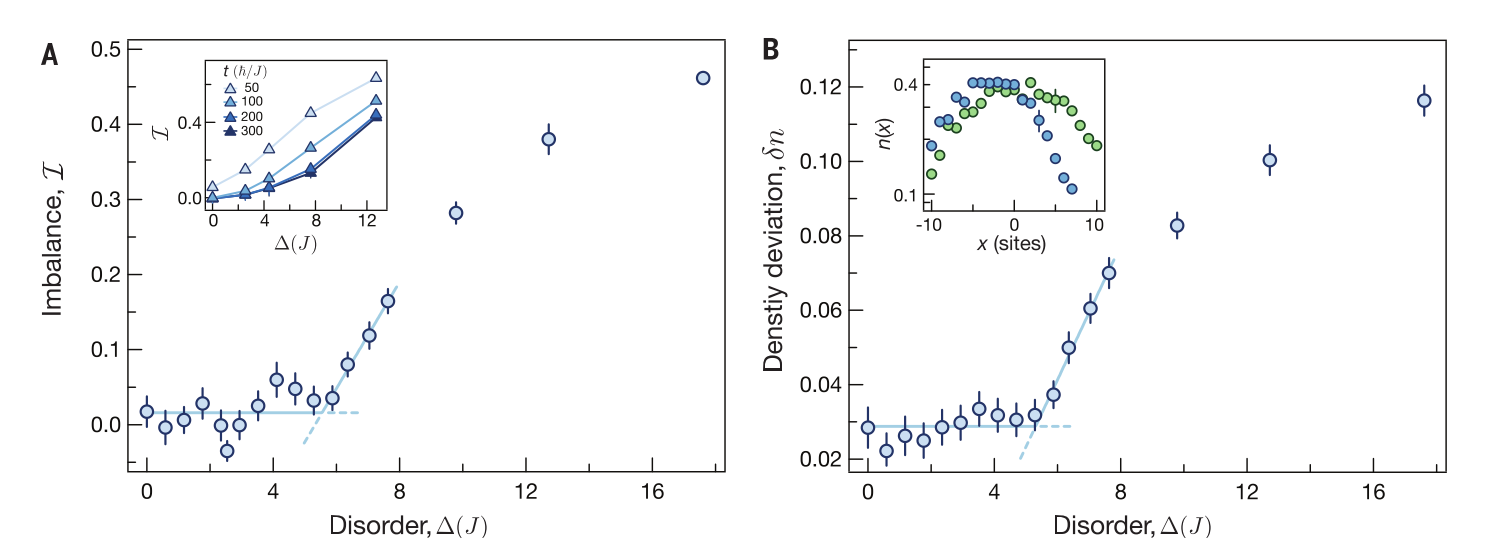
\includegraphics[width=1\linewidth]{ident}
\end{figure}
\end{frame}

\begin{frame}{Identify MBL Transition}
\small{Normalized Density:$$\bar{n}_i(\Delta) ={n}_i(\Delta)/{n}_i(0)\~e^{-\lambda(\Delta)i}$$}
\begin{figure}
 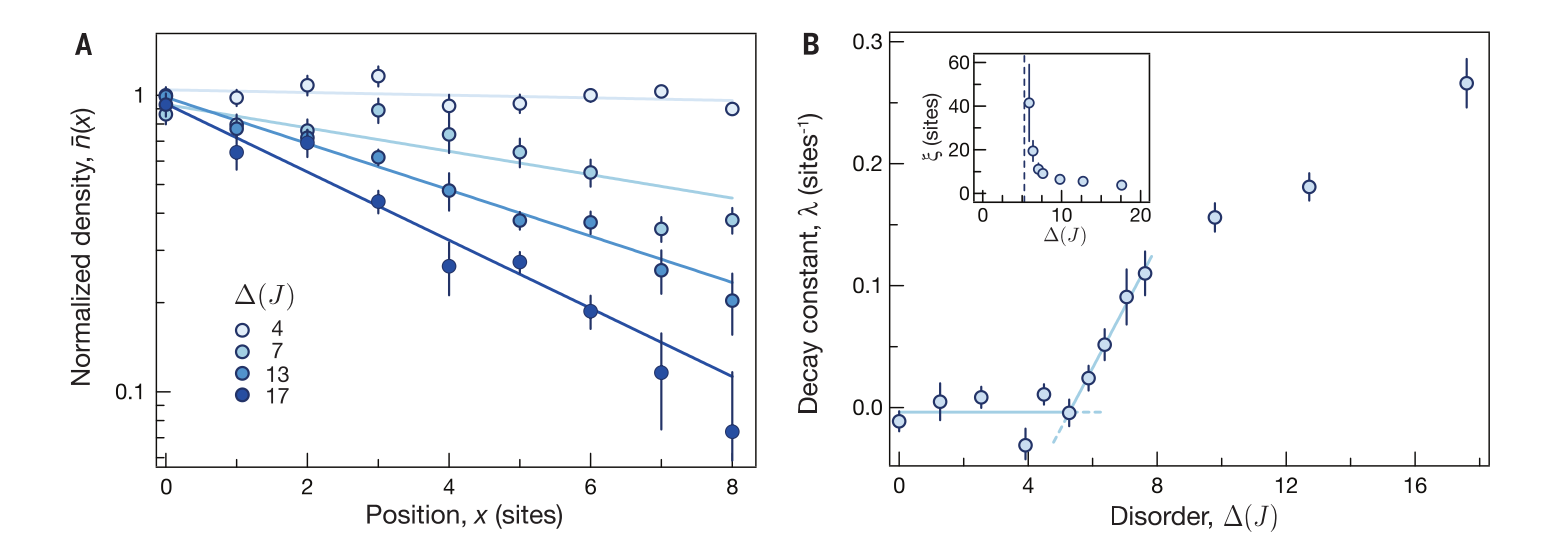
\includegraphics[width=1\linewidth]{densitydecay}
\end{figure}
\end{frame}

\begin{frame}{Effect of Interaction}
  \small{Reduce the density, therefore interaction effect.}\\~
  \small{Critical point shift can be observed,$5.3J\to3.6J$}
  \begin{figure}
   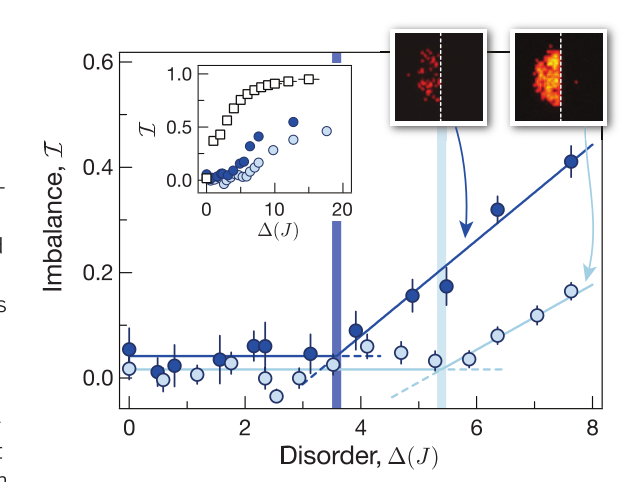
\includegraphics[width=0.6\linewidth]{inter}
  \end{figure}
\end{frame}

% \begin{frame}
% \frametitle{Table}
% \begin{table}
% \begin{tabular}{l l l}
% \toprule
% \textbf{Treatments} & \textbf{Response 1} & \textbf{Response 2}\\
% \midrule
% Treatment 1 & 0.0003262 & 0.562 \\
% Treatment 2 & 0.0015681 & 0.910 \\
% Treatment 3 & 0.0009271 & 0.296 \\
% \bottomrule
% \end{tabular}
% \caption{Table caption}
% \end{table}
% \end{frame}

% %------------------------------------------------

% \begin{frame}
% \frametitle{Theorem}
% \begin{theorem}[Mass--energy equivalence]
% $E = mc^2$
% \end{theorem}
% \end{frame}

% %------------------------------------------------

% \begin{frame}[fragile] % Need to use the fragile option when verbatim is used in the slide
% \frametitle{Verbatim}
% \begin{example}[Theorem Slide Code]
% \begin{verbatim}
% \begin{frame}
% \frametitle{Theorem}
% \begin{theorem}[Mass--energy equivalence]
% $E = mc^2$
% \end{theorem}
% \end{frame}\end{verbatim}
% \end{example}
% \end{frame}

% %------------------------------------------------

% \begin{frame}
% \frametitle{Figure}
% Uncomment the code on this slide to include your own image from the same directory as the template .TeX file.
% %\begin{figure}
% %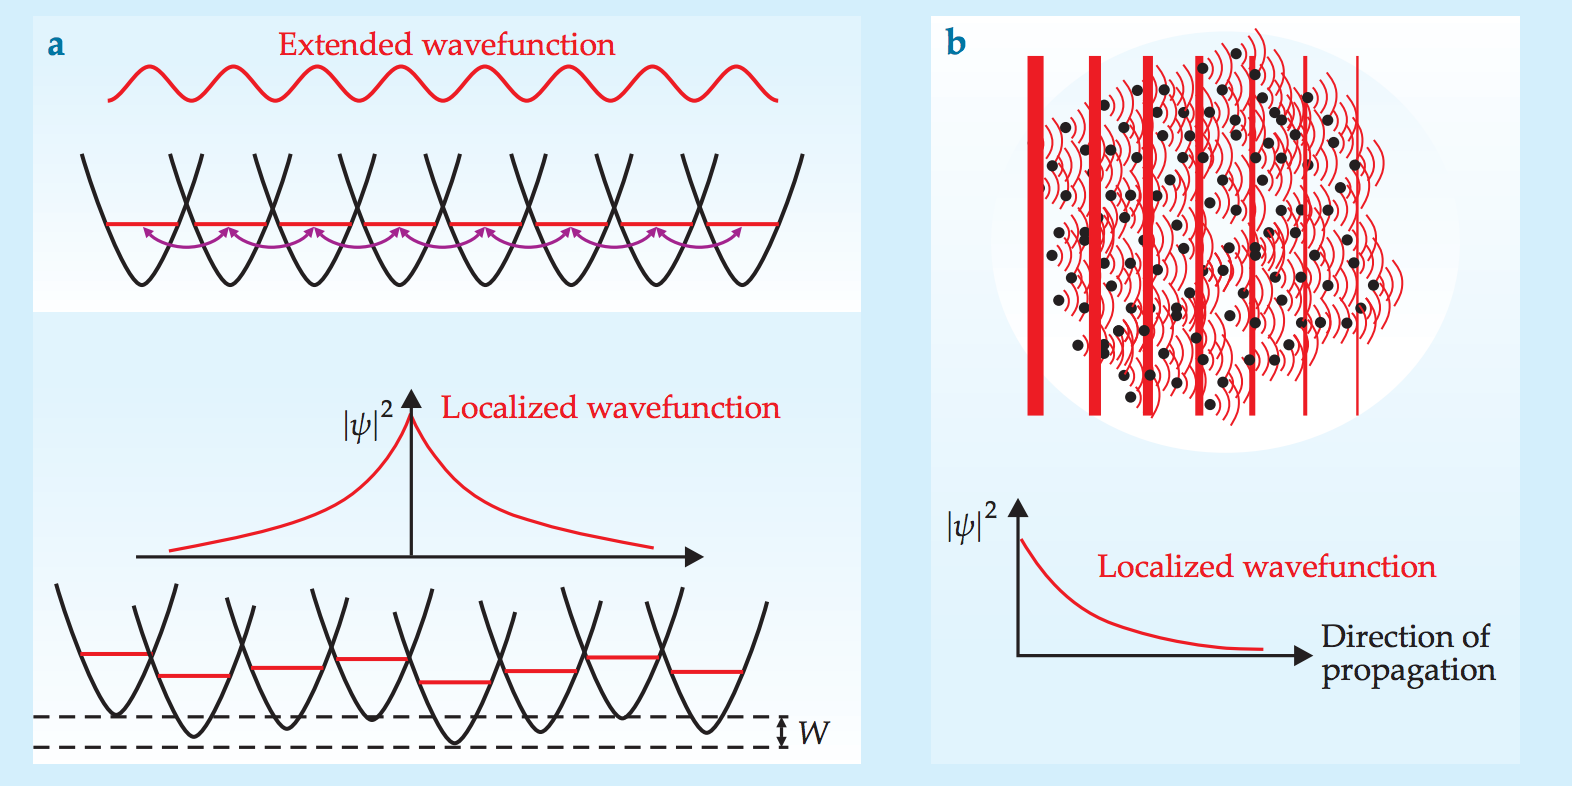
\includegraphics[width=0.8\linewidth]{AndersonLocalization.png}
% %\end{figure}
% \end{frame}

%------------------------------------------------

% \begin{frame}[fragile] % Need to use the fragile option when verbatim is used in the slide
% \frametitle{Citation}
% An example of the \verb|\cite| command to cite within the presentation:\\~

% This statement requires citation \cite{p1}.
% \end{frame}

% %------------------------------------------------参考文献的写法

% \begin{frame}
% \frametitle{References}
% \footnotesize{
% \begin{thebibliography}{99} % Beamer does not support BibTeX so references must be inserted manually as below
% \bibitem[Smith, 2012]{p1} John Smith (2012)
% \newblock Title of the publication
% \newblock \emph{Journal Name} 12(3), 45 -- 678.
% \end{thebibliography}
% }
% \end{frame}

%------------------------------------------------结尾语

\begin{frame}
\Huge{\centerline{The End}}
\end{frame}

%----------------------------------------------------------------------------------------

\end{document}
